\documentclass{article}%
\usepackage[T1]{fontenc}%
\usepackage[utf8]{inputenc}%
\usepackage{lmodern}%
\usepackage{textcomp}%
\usepackage{lastpage}%
\usepackage[head=40pt,margin=0.5in,bottom=0.6in]{geometry}%
\usepackage{graphicx}%
%
\title{\textbf{Ministro Reverol: Homicidios en Caracas han disminuido un 35,4\%}}%
\author{EFE}%
\date{11/10/2018}%
%
\begin{document}%
\normalsize%
\maketitle%
\textbf{URL: }%
http://www.eluniversal.com/sucesos/22959/ministro{-}reverol{-}homicidios{-}en{-}caracas{-}han{-}disminuido{-}un{-}354\newline%
%
\textbf{Periodico: }%
EU, %
ID: %
22959, %
Seccion: %
sucesos\newline%
%
\textbf{Palabras Claves: }%
NO\_TIENE\newline%
%
\textbf{Derecho: }%
1.10, %
Otros Derechos: %
, %
Sub Derechos: %
1.10.1\newline%
%
\textbf{EP: }%
NO\newline%
\newline%
%
\textbf{\textit{El ministro de Interiores añadió que los secuestros han disminuido en un 50\%. "Y eso es gracias a la las labores de patrullaje, de inteligencia y de labor inmediata"}}%
\newline%
\newline%
%
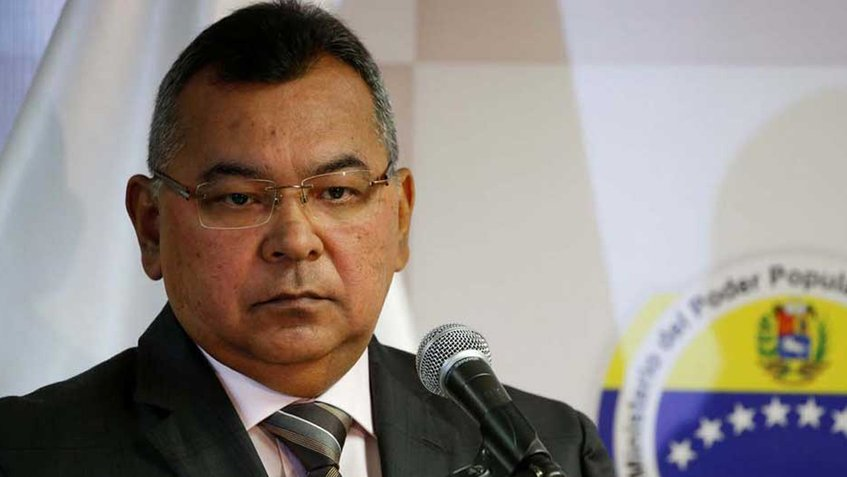
\includegraphics[width=300px]{97.jpg}%
\newline%
%
Caracas.{-}El ministro de Relaciones Interiores, Justicia y Paz, Néstor Reverol, informó este jueves que en lo que va de año los casos de homicidio han "disminuido" en un 35,4\% en Caracas, considerada una de las ciudades más violentas del mundo.%
\newline%
%
"Queremos informar que en el Distrito Capital ha habido una disminución de la incidencia delictiva, es importante destacar, de un 30,8\% en comparación al 2017 y en los homicidios ha habido una reducción importante de 35,4\%", dijo Reverol durante un despliegue de cuerpos de seguridad en un sector de la capital venezolana.%
\newline%
%
Para respaldar estos datos indicó que "por ejemplo de ayer para hoy no hubo homicidios en el Distrito Capital". \newline%
\newline%
Sin embargo, durante la mañana de este jueves un niño de 12 años murió por una bala perdida en un enfrentamiento entre la policía y delincuentes y, en otro hecho, un joven de 27 años fue asesinado para presuntamente robarle el teléfono celular, reseñó Efe.%
\newline%
%
En sus declaraciones, el ministro no hizo referencia a estos hechos ocurridos en el centro y este de Caracas, ni profundizó en detalles sobre la información que ofreció.%
\newline%
%
Reverol añadió que los secuestros han disminuido en un 50\%.~"Y eso es gracias a la las labores de patrullaje, de inteligencia y de labor inmediata", afirmó.%
\newline%
%
A finales del año pasado, Reverol informó que el número de homicidios en Venezuela se redujo en un 15,2\% al pasar de 16.976 crímenes reportados en 2016 a 14.389 en 2017.%
\newline%
%
El número oficial estuvo muy por debajo del ofrecido por la ONG Observatorio Venezolano de Violencia (OVV), que registró 89 muertes violentas por cada 100.000 habitantes, lo que se traduce en 26.616 víctimas.%
\newline%
%
\end{document}